\documentclass[11pt]{article}
\usepackage{fullpage}
\usepackage{empheq}
\usepackage{color}
\usepackage {listings}
\usepackage{amsmath}
\usepackage{hyperref}
\usepackage{longtable}
\usepackage{array}
%\usepackage[scaled]{beramono}
\usepackage[T1]{fontenc}
\usepackage{tabularx}
\usepackage{amssymb}
\usepackage{enumitem}
\usepackage{booktabs}
\usepackage{multirow} 
\usepackage{tipa}


%\setmonofont{Consolas} %to be used with XeLaTeX or LuaLaTeX
\definecolor{bluekeywords}{rgb}{0,0,1}
\definecolor{blue(munsell)}{rgb}{0.0, 0.5, 0.69}
\definecolor{greencomments}{rgb}{0,0.5,0}
\definecolor{redstrings}{rgb}{0.64,0.08,0.08}
\definecolor{xmlcomments}{rgb}{0.5,0.5,0.5}
\definecolor{types}{rgb}{0.17,0.57,0.68}
\setlength\parindent{0pt}

\lstset{language=[Sharp]C,
captionpos=b,
%numbers=left, %Nummerierung
%numberstyle=\tiny, % kleine Zeilennummern
frame=lines, % Oberhalb und unterhalb des Listings ist eine Linie
showspaces=false,
showtabs=false,
breaklines=true,
showstringspaces=false,
breakatwhitespace=true,
escapeinside={(*@}{@*)},
commentstyle=\color{greencomments},
morekeywords={partial, var, get, set,string,false,true},
keywordstyle=\color{bluekeywords},
stringstyle=\color{redstrings},
basicstyle=\ttfamily\small,
}
\lstset%
{%
    emph=[1]%
    {%
        Process,
        Cplex,
        Program,
        IntParam,
        NumVarType,
        INumVar,
        SystemInformation,
        Param,
        Stopwatch,
        Instance,
        ProcessStartInfo,
        Point,
        ILinearNumExpr,
        List,
        PathGenetic,
        Random,
        ILinearNumExpr,
        TSPLazyConsCallback,
        StreamWriter,
        IRange,
        itemList,
        DoubleParam,
        Convert,
        StringSplitOptions
    },
    emphstyle=[1]{\color{blue(munsell)}},
}


\begin{document}

ABSTRACT

\vspace{2\baselineskip}

Il presente progetto riguarda la progettazione di un software in grado di risolvere istanze del problema del Commesso Viaggiatore applicando differenti algoritmi risolutori. L'obiettivo di questo testo \`e quello di descrivere le tecniche utilizzate e di confrontare i risultati ottenuti in termini di efficienza e bont\`a della soluzione prodotta. Verr\`a fornita una descrizione degli strumenti e l'ambiente di sviluppo utilizzati e sar\`a analizzato il codice di programmazione realizzato; non mancheranno paragrafi dedicati ad approfondire concetti teorici senza i quali la comprensione del codice potrebbe risultare meno chiara. 

\vspace{2\baselineskip}
INTRODUZIONE 

\vspace{2\baselineskip}

Questa capitolo introduttivo \`e dedicato alla storia, alle applicazioni e alle correnti sfide riguardanti uno dei pi\`u importanti problemi che la disciplina di Ricerca Operativa si trova ad affrontare, ossia il problema del commesso viaggiatore(Travelling Salesman Problem-TSP). 
Il nome deriva dalla sua pi\`u tipica rappresentazione: data una rete di citt\`a, connesse tramite delle strade, si vuole trovare il percorso di minore distanza che un commesso viaggiatore deve seguire per visitare tutte le citt\`a una ed una sola volta e ritornare alla citt\`a di partenza. Per quanto detto, risulta naturale modellare il TSP come un grafo pesato i cui nodi modellizzano le citt\`a relative al problema in questione mentre i possibili collegamenti tra le localit\`a sono modellati con gli archi del grafo i cui pesi possono rappresentare,per esempio, la distanza esistente fra la coppia di nodi collegati dall' arco. Chiaramente \`e possibile assegnare i pesi in modo arbitrario secondo le nostre esigenze, ad esempio si potrebbe anche tenere conto dei tempi di percorrenza o di eventuali pedaggi presenti nei singoli percorsi. Come \`e facile immaginare, il TSP pu\`o essere quindi utilizzato per una infinit\`a  di problemi pratici ma anche teorici.\\
Il problema del commesso viaggiatore riveste un ruolo notevole nell' ambito di problemi di logistica distributiva, detti anche problemi di routing. Questi riguardano l'organizzazione di sistemi di distribuzione di beni e servizi. Esempi di problemi di questo genere sono la movimentazione di pezzi o semilavorati tra reparti di produzione, la raccolta e distribuzione di materiali, la distribuzione di merci da centri di produzione a centri di distribuzione.
Sebbene le applicazioni nel contesto dei trasporti siano le pi\`u naturali per il TSP, la semplicit\`a del modello ha portato a molte applicazioni interessanti in altre aree. Un esempio pu\`o essere la programmazione di una macchina per eseguire fori in un circuito. In questo caso i fori da forare sono le citt\`a  e il costo del viaggio \`e il tempo necessario per spostare la testa del trapano da un foro all'altro. 
Il problema del commesso viaggiatore risulta essere NP-hard: questo significa che, al momento, non \`e noto in letteratura un algoritmo che lo risolva in tempo polinomiale. Poich\`e esiste sempre una istanza per cui il tempo di risoluzione cresce esponenzialmente non \`e sempre possibile utilizzare algoritmi esatti per risolvere il TPS. Risulta quindi necessario fornire algoritmi euristici, in grado di risolvere in modo efficace istanze con un numero elevato di nodi in tempi ragionevoli.


Problemi matematici riconducibili al TSP furono trattati nell' Ottocento dal matematico irlandese Sir William Rowan Hamilton e dal matematico Britannico Thomas Penyngton.  Nel 1857, a Dublino, Rowan Hamilton descrisse un gioco, detto Icosian game, a una riunione della British Association for the Advancement of Science. Il gioco consisteva nel trovare un percorso che toccasse tutti i vertici di un icosaedro, passando lungo gli spigoli, ma senza mai percorrere due volte lo stesso spigolo. L'icosaedro ha 12 vertici, 30 spigoli e 20 facce identiche a forma di triangolo equilatero.
Il gioco, venduto alla ditta J. Jacques and Sons per 25 sterline, fu brevettato a Londra nel 1859, ma vendette pochissimo. Questo problema \`e un TSP nel quale gli archi che collegano vertici adiacenti, e quindi corrispondono a spigoli dell'icosaedro, sono consentiti e gli altri no (si pu\`o pensare che richiedano moltissimo tempo e quindi vadano sicuramente scartati), per tale ragione si tratta di un caso molto particolare di TSP. La forma generale del TSP fu invece studiata solo negli anni Venti e Trenta del ventesimo secolo dal matematico ed economista Karl Menger. Tuttavia, per molto tempo non si ebbe altra idea che quella di generare e valutare tutte le soluzioni, il che mantenne il problema praticamente insolubile. Il numero totale dei differenti percorsi possibili attraverso le $n$ citt\`a \`e facile da calcolare: data una citt\`a di partenza, ci sono a disposizione $(n - 1)$ scelte per la seconda citt\`a, $(n - 2)$ per la terza e cos\` via. Il totale delle possibili scelte tra le quali cercare il percorso migliore in termini di costo \`e dunque $(n - 1)!$, ma dato che il problema ha simmetria, questo numero va diviso a met\`a . Insomma, date n citt\`a, ci sono $\frac{(n-1)!}{2}$ percorsi che le collegano.

Solo nel 1954, George Dantzig, Ray Fulkerson e Selmer Johnson proposero un metodo pi\`u raffinato per risolvere il TSP  su un campione di $n = 49$ citt\`a: queste rappresentavano le capitali degli Stati Uniti e il costo del percorso era calcolato in base alle distanze stradali. 

Nel 1962, Procter and Gamble bandì un concorso per 33 citt\`a, nel 1977 fu bandito un concorso che collegasse le 120 principali citt\`a della Germania Federale e la vittoria and\`o a Martin Gr\"otschel oggi Presidente del Konrad-Zuse-Zentrum f\"ur Informarionstechnik Berlin(ZIB) e docente presso la Technische Universit\"at Berlin(TUB).

Nel 1987  Padberg e Rinaldi riuscirono a completare il giro degli Stati Uniti attraverso 532 citt\`a. Nello stesso periodo Groetschel e Holland trovarono il TSP ottimale per il giro del mondo che passava per 666 mete importanti. 
Nel 2001, Applegate, Bixby, Chvátal, and Cook trovarono la soluzione esatta a un problema di 15.112 citt\`a tedesche, usando il metodo cutting plane, originariamente proposto nel 1954 da George Dantzig, Delbert Ray Fulkerson e Selmer Johnson. Il calcolo fu eseguito da una rete di 110 processori della Rice University e della Princeton University. Il tempo di elaborazione totale fu equivalente a 22,6 anni su un singolo processore Alpha a 500 MHz.
Sempre Applegate, Bixby, Chv\a`tal, Cook, e Helsgaun trovarono nel Maggio del 2004 il percorso ottimale di 24,978 citt\`a della Svezia. 
Nel marzo 2005, il TSP riguardante la visita di tutti i 33.810 punti in una scheda di circuito fu risolto usando CONCORDE: fu trovato un percorso di 66.048.945 unit\`a, e provato che non poteva esisterne uno migliore. L'esecuzione richiese approssimativamente 15,7 anni CPU. 
Ai giorni nostri il risolutore Concorde per il problema del commesso viaggiatore \`e utilizzato per ottenere soluzioni ottime su tutte le 110 istanze della libreria TSPLIB; l' istanza con pi\`u nodi in assoluto ha 85,900 citt\`a. 

\vspace{2\baselineskip}

MODELLO MATEMATICO
\vspace{2\baselineskip}

Nella sua formalizzazione pi\`u generale, il problema del Commesso Viaggiatore consiste nell' individuare un circuito hamiltoniano di costo minimo in un dato grafo orientato $G=(V,A)$, dove $V = $\{$ {v_1,\dots,v_n} $\}$ $ \`e un insieme di $n$ nodi e $A = $\{$ {(i,j): i, j \in V} $\}$ $ \`e un insieme di $m$ archi. 

Senza perdita di generalit\`a, si suppone che il grafo $G$ sia completo e che il costo associato all' arco $[i,j]$, che indicheremo con $c_{ij}$, sia non negativo. Si osserva che aver imposto $c_{ij} \ge 0$ non \`e limitativo poich\'e \`e sempre possibile sommare a tutti i costi una costante sufficientemente elevata senza alterare l' ordinamento delle soluzioni. 
A differenza di quanto detto in precedenza, per tutto il proseguimento della tesi supporremmo il grafo $G$ non orientato: tale scelta deriva dal fatto che, poich\'e $c_{ij}$ nel nostro lavoro rappresenta sempre la distanza (tipicamente euclidea) fra i vertici i e j si ha che:
$$c_{ij} = c_{ji}$$

ossia il costo associato ad un arco non dipende dalla direzione dell' arco stesso. Quando il grafo \`e non orientato la famiglia di coppie non ordinate di elementi di V, ossia l' insieme degli archi, viene indicato con $E$.


Definito il problema forniamo ora una sua possibile formulazione in termini di PLI. Introducendo le seguenti variabili decisionali:

\[
x_{e}=
\begin{cases}
1 & \text{se il lato $e \in E$ viene scelto nel circuito ottimo} \\
0 & \text{altrimenti}
\end{cases}
\]

si ottiene il problema:

\begin{eqnarray}
& \text{min}\displaystyle\underbrace{\sum_{e \in E} c_e x_e}_{\text{costo circuito}} \\[1.5ex]
&\displaystyle\underbrace{\sum_{e \in \delta(V)} x_e = 2}_{\text{due lati incidenti in }v}\text{,  }\forall v \in V \\[1.5ex]
&0\leq x_e \leq 1 \text{ intera , }\forall e \in E
\end{eqnarray}

L' insieme di vincoli definiti dalla (2) vengono chiamati vincoli di grado e impongono che in ogni vertice incidono esattamente due lati. In questa forma il modello \`e  compatto dato che il numero di vincoli \`e polinomiale rispetto alla dimensione dell' istanza ma non \`e completo poich\'e \`e sprovvisto dei vincoli di subtour che impediscono alla soluzione ottima di avere dei subtour al suo interno.

\begin{center}
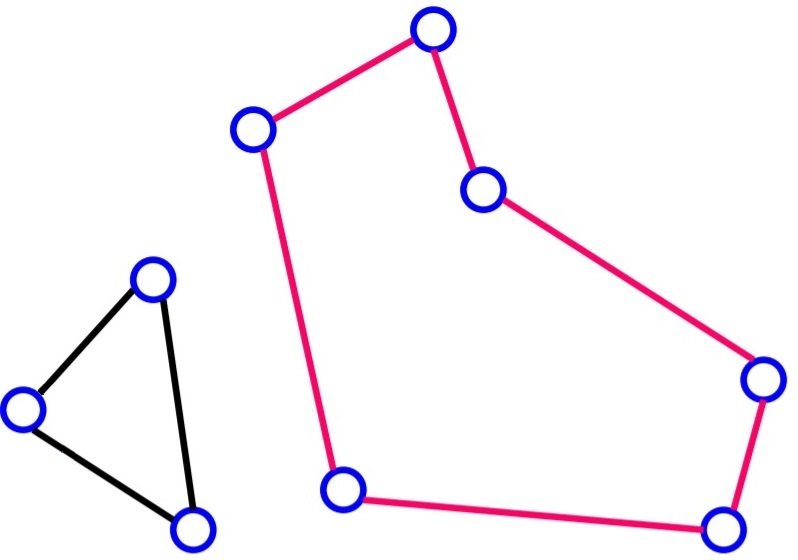
\includegraphics[scale=0.5]{subtour}  

Figura 1: Soluzione con due subtour
\end{center}

\vspace{2\baselineskip}

Una possibile formulazione per i vincoli di subtour risulta essere:

\begin{eqnarray}
&\displaystyle{\sum_{e \in E(S)}x_e \geq 1} \text{ , } \forall S \subsetneq V \text{ : } 1 \in S \text{ , } |S| \geq 2
\end{eqnarray}


Il vincolo (4) indica che se si considera un sottoinsieme $S \subsetneq V$, che includa il vertice numerato con il simbolo 1, allora il taglio di G indotto da S:

\begin{center}
$\delta(S) = $\{$ {[i,j]\in E : i \in S, j \notin S} $\} $ $
\end{center}

deve contenere almeno un lato appartenente ad $E$: poich\'e tutti i subtour violano tale vincolo la soluzione ottima non potr\`a contenere subtour al suo interno.  
Essendo il numero di vincoli di subtour pari al numero di sottoinsiemi $S$ distinti, il numero di tali vincoli risulta esponenziale rispetto alla dimensione dell' istanza. In particolare il numero di sottoinsiemi $S$ distinti che si possono formare con $n$ nodi \`e $2^n$: questo perch\`e associando un bit per ogni vertice (il cui valore definisce se appartiene o meno al sottoinsieme) un sottoinsieme S risulta identificato da una sequenza di $n$ bit e quindi si hanno $2^n$ possibili sottoinsimi $S$ distinti. Dato che si \`e imposto che il vertice 1 appartiene sempre ad ogni $S$ e che $S \subsetneq V$, si ha che il numero di vincoli di subtour risultano pari a  $2^{n-1} - 1$.

Una seconda formulazione equivalente per esprimere i vincoli di subtour \`e la seguente:

\begin{eqnarray}
&\displaystyle{\sum_{e \in E(S)}x_e \leq |S| - 1} \text{ , } \forall S \subsetneq V \text{ , } |S| \geq 2
\end{eqnarray}

I vincoli di subtour non sono stati aggiunti al modello per via del loro numero: sar\`a nostra cura progettare un opportuno separatore, ossia una funzione che fornita in ingresso una soluzione x* ottima per il modello corrente generi tutti i vincoli di subtour che verranno aggiunti "al volo" al modello.


\vspace{2\baselineskip}
LETTURA FILE DI INPUT
\vspace{2\baselineskip}


Le istanze del problema del Commesso Viaggiatore che sono state fornite in input al programma sono state selezionata da un libreria di istanze che si trovano al seguente indirizzo web: 

\begin{center}
\href{http://elib.zib.de/pub/mp-testdata/tsp/tsplib/tsp/index.html}{http://elib.zib.de/pub/mp-testdata/tsp/tsplib/tsp/index.html}
\end{center}

Tali istanze, memorizzate ciascuna in un file di testo, hanno un formato ben preciso grazie al quale \`e stato possibile progettare un opportuno parser al fine di popolare le strutture dati interne del programma con i dati presenti in tale file.
Conoscendo preventivamente la struttura del file si sono, in fase di progettazione, limitati i controlli inerenti a possibili modifiche riguardanti la struttura stessa del file, supponendo che l' utente fornisca in input solo file aventi la struttura nativa. 

\vspace{2\baselineskip}



\vspace{2\baselineskip}
STRUTTURA DEL PROGETTO
\vspace{2\baselineskip}


I file che compongono il programma realizzato sono stati organizzati nel modo seguente; all' interno della cartella TSPCsharp si sono create le seguenti sottocartelle:

\begin{itemize}
\item Src contiene i codici sorgenti scritti in C\# e l'eseguibile;
\item Data include le istanze del problema del commesso viaggiatore appartenenti alla TSPlib;
\item Concorde la quale contiene i file sorgenti in  linguaggio C del programma Concorde la cui trattazione \`e rimandata al Capitolo X.
\end{itemize}

Il software sviluppato \`e composto da dieci classi, riportiamo di seguito il nominativo di ogni classe:

\begin{itemize}
\item Instances
\item ItemList
\item PathGenetic
\item PathStandard
\item Point
\item Program
\item Tabu
\item TSP
\item TSPLazyConsCallback
\item Utility
\end{itemize}

Per le classi Point, Instances, Program, TSP e Utility verr\`a fornita una descrizione in questo capitolo, le rimanenti classi verranno presentate nei capitoli successivi poich\'e una loro trattazione risulta in questo momento prematura. 


\vspace{2\baselineskip}
CLASSE POINT
\vspace{2\baselineskip}

La classe Point \`e stata realizzate al fine di memorizzare le coordinate di un nodo appartenente all' istanza del problema del Commesso Viaggiatore fornito in ingresso al programma. Tale classe presenta due variabili private di tipo double chiamate rispettivamente x e y necessarie rispettivamente per memorizzare la coordinata x e la coordinata y del nodo. Il costruttore della classe semplicemente setta queste due variabili ai valori del nodo letto dal file di input. 

Il metodo Distance \`e l' unico metodo appartenente a questa classe ed \`e stato implementato per  calcolare il costo del lato congiungente due vertici del grafo; la sua firma \`e:

\begin{lstlisting}
    public static double Distance(Point p1, Point p2, string pointType)
\end{lstlisting}

\begin{itemize}
\item p1: Rappresenta il primo nodo;
\item p2: Rappresenta il secondo nodo;
\item pointType: Rappresenta il modo con cui il costo relativo al lato che congiunge p1 con p2 viene calcolato; i valori che questo parametro pu\`o assumere sono i seguenti:
	\begin{itemize}
	\item EUC\char`_2D
	\item ATT
	\item MAN\char`_2D
	\item GEO
	\item MAX\char`_2D	
	\item CEIL\char`_2D
	\end{itemize}
\end{itemize}

A titolo di esempio riportiamo il codice realizzato nel caso in cui pointType risulti uguale a EUC\char`_2D, in questo caso il costo del lato risulta pari alla distanza euclidea dei due nodi. 

\begin{lstlisting}

 double xD = p1.X - p2.X;
 double yD = p1.Y - p2.Y;
 
 if (pointType == "EUC_2D")
 {
     return (int)(Math.Sqrt(xD * xD + yD * yD) + 0.5);
 }
 else if ...
            
\end{lstlisting}

Per quanto riguarda gli altri metodi di calcolo della distanza rimandiamo il lettore alla visione del codice.

\vspace{2\baselineskip}
CLASSE INSTANCE
\vspace{2\baselineskip}

La classe Instance \`e stata creata per  memorizzare tutti i dati caratterizzanti l' istanza del problema del Commesso Viaggiatore. La tabella sottostante fornisce un elenco di variabili ed array definite all' interno della classe assieme ad una breve descrizione. 


\begin{center}

    \begin{longtable}{ | p{4cm} | p{4cm} | p{7cm} |}
    \hline
    \begin{center} \textbf{Tipo di dato} \end{center} & \begin{center}  \textbf{Nome} \end{center}& 
    \begin{center} \textbf{Descrizione} \end{center}\\ \hline
    \begin{center} int \end{center} & \begin{center} nNodes \end{center}& \vfill Rappresenta il numero di nodi dell' istanza del problema del Commesso Viaggiatore.\vfill \\ \hline
    \begin{center} Point[ ] \end{center} & \begin{center} coord \end{center}& \vfill Vettore di Point contenente le coordinate di tutti i vertici del grafo.\vfill\\ \hline
    \begin{center} string \end{center} & \begin{center} edgeType \end{center}&\vfill Definisce la modalit\`a con cui calcolare la distanza fra due nodi.\vfill \\ \hline
    \begin{center} double \end{center} & \begin{center} timeLimit \end{center}& \vfill Definisce la quantit\`a massima di tempo che il programma dispone per il calcolo della soluzione.\vfill \\ \hline
    \begin{center} double \end{center} & \begin{center} inputFile \end{center}&\vfill Rappresenta il nome del file di input contenente l'istanza del problema del Commesso Viaggiatore. \vfill\\ \hline
    \begin{center} double \end{center} & \begin{center} tStart \end{center}& \vfill ? \vfill \\ \hline
    \begin{center} double \end{center} & \begin{center} zBest \end{center}& \vfill Rappresenta il costo della soluzione ottima restituira da cplex.\vfill \\ \hline
    \begin{center} double \end{center} & \begin{center} tBest \end{center}& \vfill Contiene la qantit\`a di tempo impiegata per il calcolo della soluzione ottima. \vfill \\ \hline
    \begin{center} double \end{center} & \begin{center} bestSol \end{center}& \vfill Rappresenta la soluzione ottima ritornata da Cplex.\vfill \\ \hline
     \begin{center} double \end{center} & \begin{center} bestLb \end{center}& \vfill Rappresenta il miglior lower bound attualmente calcolato.\vfill \\ \hline
    \begin{center} double \end{center} & \begin{center} bestLb \end{center}& \vfill Rappresenta il miglior lower bound attualmente calcolato.\vfill \\ \hline
     \begin{center} double \end{center} & \begin{center} bestLb \end{center}& \vfill Rappresenta il miglior lower bound attualmente calcolato.\vfill \\ \hline
     \begin{center} double \end{center} & \begin{center} dMin \end{center}& ?\\ \hline
     \begin{center} double \end{center} & \begin{center} dMax \end{center}& ? \\ \hline
    \end{longtable}
\end{center}

\textit{Anzich\`e definire xMin/yMin e xMax/yMax definirei dMin e dMax. Se preferisci tenerle separate non ci sono problemi :)Il codice comunque non lo ho modificato. \\ In piu sarebbe piu giusto chiamare zBest xBest perche ascoltando le reg ho capito che la z ci andava nel suo esempio non nel nostro.. \\ mi sono accorto anche che sizePopulation non centra davvero nulla con inst e quindi la toglierei da qui}


Questa classe \`e risultata particolarmente utile poich\'e, passando come parametro una sua istanza ad un metodo,  quest' ultimo ha accesso a tutte le variabili elencate nella tabella. Non avere questa classe significava dover passare molti pi\`u parametri alle funzioni rendendo il codice meno chiaro.
L' unico metodo appartenente a questa classe risulta essere il metodo Print, la cui firma risulta essere:

\begin{lstlisting}
                  static public void Print(Instance inst)
\end{lstlisting}

dove:

\begin{itemize}
\item inst: oggetto della classe Instance contente tutti dati che descrivono l' istanza del probelma del Commesso Viaggiatore fornita in ingresso dall' utente;
\end{itemize}

Tale metodo semplicemte stampa a video le coordinate di tutti i nodi contenuti nell' array Point dell' oggetto inst. Per scrupolo viene di seguito riportato il codice:

\begin{lstlisting}
for (int i = 0; i < inst.NNodes; i++)
    Console.WriteLine("Point #" + (i + 1) + "= (" + inst.Coord[i].X + "," + inst.Coord[i].Y + ")");
\end{lstlisting}

\vspace{2\baselineskip}
CLASSE TSP
\vspace{2\baselineskip}

La classe TSP contiene il metodo TSPOpt invocato dal metodo Main e tutti gli algoritmi di risoluzione realizzati. In particolare il metodo TSPOpt realizza l'interfaccia grafica che consente all' utente di invocare l' algoritmo risolutore desiderato; nel caso in cui non si siano registrate anomalie, la funzione ritorna il valore true, viceversa false. 
\textit{[In realt\`a da noi ritorna sempre true..sarebbe meglio tornasse false in qualche caso] \\ se dici questo è anche un buon punto per dire due parole sull' interfaccia grafica creata..}

\vspace{2\baselineskip}
CLASSE UTILITY
\vspace{2\baselineskip}

La classe Utility comprende al suo interno il codice di tutti i metodi invocati dagli algoritmi risolutori presenti nella classe TSP: si \`e deciso di dirottare in questa classe tali funzioni per avere nella classe TSP un codice pi\`u leggibile.

\vspace{2\baselineskip}

CLASSE PROGRAM

\vspace{2\baselineskip}

La classe Program contiene il metodo Main che, come noto, rappresenta il punto di inizio del programma: dal sistema operativo riceve in input l' array argv di stringhe contenente i parametri inseriti dall' utente da riga di comando. Appartengono a questa classe anche i metodi ParseInst e Populate; tali metodi consentono di popolare i campi associati all' istanza (che come vedremo \`e stata chiamata inst) della classe Istance. Mentre ParseInst svolge il suo compito utilizzando i valori passati dall' utente da riga di comando, Populate utilizza i dati presenti nel file di testo contenente l' istanza del problema del Commesso Viaggiatore. Firma e implementazione di tali metodi \`e rimandata al successivo capitolo.\\
Nel metodo Main  principalmente si crea una istanza della classe Instance e si invocano nell' ordine i metodi ParseInst, Populate e TSPOpt. Nel caso non si siano rivelate anomalie e l' utente abbia scelto di utilizzare un algoritmo esatto, viene stampato a video il tempo impiegato da Cplex per il calcolo della soluzione ottima; nel caso in cui l' utente abbia scelto un algoritmo euristico viene stampato il tempo impiegato da quest' ultimo per produrre la soluzione(che non necessariamente \`e quella ottima) fornita in output.\textit{[Questa separazione non la facciamo ma secondo me \`e da fare perch\`e se usiamo un euristico e poi a video stampiamo "la soluzione ottima \`e stata trovata in..." \`e sbagliato]}. Si osserva che la stampa a video della soluzione ottima o della miglior soluzione trovata fino a quel momento nel caso di algoritmi euristici, viene effettuata all' interno dell' algoritmo risolutore.

Nella seguente tabella sono mostrate le variabili definite in questa classe assieme ad una breve descrizione. Poich\'e tali variabili sono costanti, \`e riportato pure il loro valore. 

\begin{center}

    \begin{tabular}{ | p{1.5cm} | p{4cm} | p{2cm} | p{6.5cm} |}
    \hline
    \begin{center} \textbf{Tipo di dato} \end{center} & \begin{center}  \textbf{Nome} \end{center}& \begin{center} \textbf{Valore} \end{center} & \begin{center} \textbf{Descrizione} \end{center}\\ \hline
    \begin{center} int \end{center} & \begin{center} VERBOSE \end{center}& \begin{center} 5 \end{center} & Regola quanto output il programma mostra a video: si \`e scelto di condizionare l' esecuzione di molte righe di codice che producevano una stampa a video in base al valore assunto da questa variabile. Si \`e deciso di ristringere il suo valore da 1 a 9, quando assume il valore 9 viene riportato a video il maggior numero possibile di stampe. \\ \hline
    \begin{center} int \end{center} & \begin{center} TICKS\char`_PER\char`_SECOND \end{center} &  \begin{center}1000  \end{center}& ? \\ \hline
    
\end{tabular}
\end{center}

\textit{ci sarebbe pure clock, non so se ti sei dimenticato di toglierla o \`e giusto lasciarla globale}


\vspace{2\baselineskip}
INTERPRETAZIONE FILE DI INPUT
\vspace{2\baselineskip}

Lo sviluppo del programma \`e iniziato realizzando una opportuna funzione per interpretare correttamente i parametri di ingresso forniti dall' utente. Oltre al nome del file di testo contenente i dati relativi  all' istanza del problema che si vuole risolvere, all' utente \`e richiesto di fornite un time limit(espresso in secondi) e di scegliere con quale algoritmo risolvere l'istanza da esso fornita. Si \`e deciso di ricevere da riga di comando il nome del file e il time limit; per quanto riguarda la scelta dell' algoritmo risolutore ed eventuali parametri da esso richiesti si \`e preferito realizzare una semplice interfaccia grafica per favorire l'utente. 
Per ottenere una maggiore flessibilit\`a , si \`e deciso che il valore di un parametro inserito da riga di comando  dovr\`a essere preceduto da una stringa identificatrice di quest' ultimo: in particolare si \`e deciso che il nome del file dovr\`a essere preceduto dalla stringa -file mentre il time limit dovr\`a essere preceduto dalla stringa -timelimit; questo permette di realizzare un codice che consente all' utente di  inserire in un ordina arbitrario tali parametri essendo sempre cosciente di quale parametro ha settato. Si osserva che allo stato attuale del programma il vantaggio \`e relativo passando solo due parametri ma, nel caso di futuri aggiornamenti che prevedono l' inserimento di un numero maggiore di parametri da riga di comando, il vantaggio diventerebbe notevole.
La funzione che interpreta correttamente gli argomenti forniti in input dalla riga di comando \`e stata chiamata ParseInst ed ha la seguente intestazione:

\begin{lstlisting}
	  static void ParseInst(Instance inst, string[] input)    

\end{lstlisting}


\begin{itemize}
\item inst: rappresenta un riferimento l'istanza della classe Instance contente tutti dati che descrivono l' istanza del probelma del Commesso Viaggiatore fornita in ingresso dall' utente;
\item input: rappresenta un vettore contenente i parametri di input forniti da riga di comando dall' utente.
\end{itemize}


Il metodo \`e composto da un ciclo for il quale scandisce ad ogni iterazione tutte le celle dell'array input: se \`e presenta una uguaglianza fra l' elemento $i$ dell' array e una stringa identificatrice si assegna ad una opportuna variabile di inst il relativo valore che si trova in input[i+1]. Successivamente si esegue l'istruzione continue in modo da interrompere il corrente ciclo per iniziare il successivo.

\begin{lstlisting}

for (int i = 0; i < input.Length; i++)
{
   if (input[i] == "-file")
   {
     //Expecting that the next value is the file name
       inst.InputFile = input[++i];
       continue;
    }
    if (input[i] == "-timelimit")
    {
      //Expecting that the next value is the time limit in seconds
       inst.TimeLimit = Convert.ToDouble(input[++i]);
       continue;
    }
}   			
\end{lstlisting}

Nel caso in cui l' utente non fornisca il nome del file di input oppure il time limit viene lanciata una eccezione:

\begin{lstlisting}

if (inst.InputFile == null || inst.TimeLimit == 0)
     throw new Exception("File input name and/or timelimit are missing");

\end{lstlisting}


\vspace{2\baselineskip}
METODO POPULATE
\vspace{2\baselineskip}

Come gi\`a accennato, il metodo Populate \`e stato implementato per memorizzare tutte le informazioni relative all' istanza del problema del Commesso Viaggiatore contenute nel file di testo nei rispettivi campi presenti in inst.
Essendoci dati di natura diversa all' interno del file, quest' ultimo \`e diviso in sezioni che cominciano con una parola chiave. Tranne la sezione che inizia con la parola chiave NODE COORD SECTION, tutte le altre si sviluppano in una sola riga la quale ha la seguente struttura:

\begin{center}
<parolaChiave> : < valore> 
\end{center}

Di seguito sono riportati i valori che possono essere assunti dalle parole chiavi e il significato del contenuto della relativa sezione: 

\begin{itemize}
	\item NAME:<string> 
	\begin{itemize}
	\item nome con cui l' istanza \`e nota in letteratura.
	\end{itemize}
	\item TYPE:<string>
	
	\begin{itemize}	 
	\item indica il tipo dell' istanza. Nel nostro ambito sar\`a sempre TSP.    
    \end{itemize}	
	 
	\item COMMENT:<string> 
	\begin{itemize}	
	\item include informazioni aggiuntive, solitamente contiene il nome deli gli autori che hanno proposto l'  				istanza.
	\end{itemize}	
	
		
	\item DIMENSION:<integer> 
	\begin{itemize}
	\item indica il numero di nodi.
	\end{itemize}	
	
	\item EDGE WEIGHT TYPE:<string>
	\begin{itemize} 
	\item Definisce il modo con cui il costo del lato deve essere calcolato, i possibili valori  che pu\'o assumere    		     il contenuto di questa sezione sono stati gi\`a presentati a pagina 7 durante la descrizione del metodo Distance.
	\end{itemize}	
	
	\item NODE COORD SECTION: 
	\begin{itemize}	
	
	\item Il contenuto di questa sezione si sviluppa in pi\`u righe; in ogni riga troviamo nell' ordine:
	\begin{itemize}
	\item Un numero progressivo intero positivo che comincia da 1 e che identifica il nodo. Osserviamo che anche se in input il       
	primo nodo \`e numerato a partire da 1, nel vettore Point di inst le coordinate saranno memorizzate a partire dall' indice 0. 		In ogni caso sar\`a nostra cura quando ci interfacciamo con l' utente far partire la numerazione dei nodi da 1.
	\item Un numero reale positivo che definisce la coordinata x del nodo.
	\item Un numero reale positivo che identifica la coordinata y del nodo.
	\end{itemize}		
	\end{itemize}	
\end{itemize}

Il file di testo termina sempre con la stringa EOF che indica la fine del file di testo.

Per poter leggere il contenuto di un file \`e necessario inizializzare una nuova istanza della classe StreamReader passando come parametro al costruttore il percorso ove tale file \`e  collocato.


\begin{lstlisting}

StreamReader sr = new StreamReader("..\\..\\..\\..\\Data\\" + inst.InputFile)

\end{lstlisting}


Il metodo ReadLine() della classe StreamReader ritorna, come stringa, il contenuto di una intera riga del file la quale viene memorizzata all' interno di una variabile di tipo string chiamata line. Poich\'e si vuole leggere tutto il contenuto del file, \`e necessario invocare ReadLine() ciclicamente sull' oggetto sr creato finch\`e line risulta diversa da null. Quando line risulta pari a null significa che il file \`e terminato e quindi tutto il suo contenuto \`e stato letto.

Per quanto detto si \`e realizzato il seguente ciclo while per scandire tutte le righe del file:

\begin{lstlisting}

while ((line = sr.ReadLine()) != null)
{
	...
}
\end{lstlisting}


Poich\'e ogni riga inizia con una nota parola chiave, per prelevare il contenuto di una sezione e memorizzarlo in un opportuno campo di inst, \`e sufficiente confrontare la prima stringa di ogni riga con una delle noti parole chiavi. Per far ci\`o si \`e  usato il metodo StartWith della classe String, la cui firma \`e:

\begin{lstlisting}

                    public bool StartWith(string value)

\end{lstlisting}

Questo metodo, applicato alla variabile line, determina se la prima stringa di line corrisponde alla stringa value specificata all' atto dell' invocazione del metodo. In caso in cui il confronto dia esito positivo, per prelevare il contenuto della sezione \`e neccessario applicare i metodi IndexOf e Remove sempre alla variabile line; l' intestazione di tali metodi \`e riportata di seguito:


\begin{lstlisting}

               public int IndexOf(string value,int startIndex)

\end{lstlisting}

dove:

\begin{itemize}
	\item value: stringa da cercare;
	\item startIndex: posizione iniziale della ricerca.
\end{itemize}

\begin{lstlisting}

                public string Remove(int startIndex, int count)

\end{lstlisting}


dove:

\begin{itemize}
	\item startIndex: posizione in base zero da cui iniziare l'eliminazione dei caratteri;
	\item count: numero di caratteri da eliminare.
\end{itemize}

Per quanto visto, risulta immediata la comprensione del codice neccssario per prelevare il contenuto della sezione e memorizzarlo in un generica variabile, chiamata campo:

\begin{lstlisting}

                inst.campo = (line.Remove(0, line.IndexOf(:) + 2));

\end{lstlisting}

Si ritiene utile osservare che \`e stato necessario incrementare il valore ritornato da meodo IndexOf di 2 poich\'e \`e presenta uno spazio fra il carattere ":" e il contenuto della sezione.

Nel caso in cui campo non \`e di tipo string \`e necessario effettuare una conversione esplicita utilizzando i metodi ToInt o ToDouble della classe Convert: questo in ogni caso non \`e un problema poich\'e noto il tipo di dato contenuto di una sezione.

Poich\'e  il contenuto della sezione NODE COORD SECTION si sviluppa in pi\`u righe, si \`e dichiarata una variabile di tipo bool chiamata readingCoordinates inizializzata al valore logico false; a questa variabile viene assegnato il valore logico true solo una volta che si \`e entrati in questa sezione. 
Per leggere il contenuto di questa sezione si \`e realizzato un if la cui condizione valutava se readingCoordinates assumeva il valore logico true; in tal caso sono eseguite le seguenti istruzioni:

\begin{lstlisting}

string[] elements = line.Split(new[]{ ' ' } , StringSplitOptions.RemoveEmptyEntries);

int i = Convert.ToInt32(elements[0]);

inst.Coord[i - 1] = new Point(Convert.ToDouble(elements[1].Replace(".", ",")), Convert.ToDouble(elements[2].Replace(".",",")));
\end{lstlisting}

Il metodo Split della classe String ritorna un array contenente in ogni elemento una sottostringa della stringa a cui tale metodo \`e applicato. Le sottostringhe vengono estratte dalla stringa in base ai caratteri delimitatori specificati all' atto dell'invocazione del metodo, quest' ultimo ha diversi overload: quello di nostro interesse \`e riportato di seguito.

\begin{lstlisting}

     public string[] Split(char[] separator, StringSplitOptions options)

\end{lstlisting}

dove:

\begin{itemize}
\item separator: array i cui elementi definiscono i separatori della stringa. 
\item options: A questo parametro possono essere passate solo i seguenti due valori dell' enumerazione StringSplitOptions:

\begin{itemize}

\item StringSplitOptions.RemoveEmptyEntries: indica che gli elementi dell' array ritornato non possono essere stringhe vuote.
\item StringSplitOptions.None: indica che gli elementi dell' array ritornato possono essere stringhe vuote.

\end{itemize}

\end{itemize}

Nel nostro caso dato che l' unico separatore \`e lo spazio vuoto, \`e stato sufficiente passare come primo parametro a Split un array con un solo elemento contenente il carattere \textipa{"}   \textipa{"}.
Successivamente all' interno di una variabile di tipo intero chiamata i si \`e memorizzato l' indice del nodo che, per quanto visto, \`e memorizzato sempre in elements[0] ed \`e un numero intero: per tale ragione \`e stato necessario applicare il metodo ToInt32 della classe Convert.
Si \`e infine memorizzato nel vettore Coor di inst, in un oggetto Point,le coordinate del nodo presenti in elements[1] e elements[2]. Come accennato in precedenza, mentre la numerazione dei nodi nell' istanza parte da 1, la memorizzazione delle coordinate in Coor inizia dall' indice 0.

Anche in questo caso \`e stato necessario effettuare una conversione da string a double ; inoltre \`e stato doveroso utilizzare il metodo Replace della classe string avente la seguente firma:

\begin{lstlisting}

     public string Replace(string oldValue, string newValue
)

\end{lstlisting}
dove:
\begin{itemize}
	\item oldValue: stringa sa sostituire;
	\item newValue: stringa con cui sostituire tutte le occorrenze di oldValue.
\end{itemize}


Questo perch\`e il generale le coordinate dei vertici sono numeri reali aventi come carattere di separazione fra la parte intera e quella decimale il carattere \textipa{"}.\textipa{"} anzich\`e il carattere \textipa{"},\textipa{"} : questo fatto genera anomalie nella conversione fra i tipi di dato string e double e quindi \`e  stato necessario effettuare tale sostituzione di caratteri.


\vspace{2\baselineskip}
COSTRUZIONE DEL MODELLO
\vspace{2\baselineskip}

In questo paragrafo vedremo come \`e possibile creare da programma un modello matematico attraverso l' uso di alcune routine appartenenti alla libreria di Cplex. Premettiamo che esula dallo scopo di questa tesi fornire al lettore una descrizione del funzionamento di Cplex da iterativo.


\vspace{2\baselineskip}
COSTRUZIONE MODELLO IN C
\vspace{2\baselineskip}

Per istanziare un nuovo modello di programmazione lineare \`e necessario inizializzare un enviroment di Cplex utilizzando la funzione CPXopenCPLEX la quale ritorna un puntatore all' envairoment creato, la firma di tale funzione \`e:


\begin{lstlisting}

                CPXENVptr CPXopenCPLEX(int* status_p)

\end{lstlisting}

dove:

\begin{itemize}
\item status\char`_p: puntatore ad una variabile di tipo intero usato per ritornare un eventuale codice di errore.
\end{itemize}


L' enviroment \`e una struttura dati interna a Cplex i cui dettagli implementativi non sono di dominio pubblico, contenente variabili inerenti all' esecuzione di Cplex. Per esempio variabili interne all' enviroment sono il time limit e la variabile verbose. Ad un enviroment possiamo associare uno o pi\`u modelli: per associare un modello \`e necessario usare il metodo CPXcreateprob, la cui intestazione \`e:

\begin{lstlisting}

    CPXLPptr CPXcreateprob(CPXCENVptr env, int * status_p, const char * probname_str)


\end{lstlisting}


dove:

\begin{itemize}
	\item env: puntatore all' environment sul quale si \`e deciso di creare il modello;
	\item status\char`_p: puntatore ad una variabile di tipo intero usato per ritornare un eventuale codice di errore;
	\item probname\char`_str: rappresenta un array di caratteri che definisce il nome del modello creato.
\end{itemize}

Tale funzione ritorna un puntatore al modello creato: questo risulta vuoto poich\`e  privo di funzione obbiettivo, di variabili e di vincoli.\\

Per poter definire la funzione obbiettivo \`e necessario aggiungere tutte le variabili definendo per ciascuna il relativo costo; un primo metodo per far ci\`o \`e inserire contemporaneamente tutte le variabili utilizzando la funzione CPXnewcols la cui firma \`e:


\begin{lstlisting}

int CPXnewcols (CPXENVptr env,CPXLPptr lp,int ccnt,double *obj, double *lb, double *ub, char *ctype, char **colname);

\end{lstlisting}

dove:

\begin{itemize}
\item env : puntatore all' enviroment di Cplex nel quale vuole essere inserito il modello.
\item lp : puntatore al problema di programmazione lineare.
\item ccnt : intero che indica il numero delle nuove variabili che vengono aggiunte al problema.
\item obj : array contenente per ogni variabile il relativo coefficiente 
\item lb : array di lunghezza ccnt contenente il lower bound di ogni variabile aggiunta.
\item ub : array contenente l' upper bound di ogni variabile aggiunta.
\item ctype : array di lunghezza ccnt contenente il tipo di ogni variabile. I valori che un elemento di questo array pu\`o assumere sono:
\begin{itemize}
	\item \textipa{"}C\textipa{"}: variabile continua
	\item \textipa{"}B\textipa{"}: variabile binaria
	\item \textipa{"}I\textipa{"}: variabile intera
\end{itemize}
\item colname : array di lunghezza ccnt contenente puntatori ad array di char contenente ogniuno il nome della variabile aggiunta al modello.
\end{itemize}

A livello implementativo \`e risultato pi\`u semplice anzich\`e  aggiungere al modello tutte le variabili contemporaneamente, utilizzare un secondo approccio che consiste nell' inserire una variabile per volta invocando la funzione CPXnewcols tante volte quante sono le variabili da aggiungere. In particolare si \`e inserita la funzione CPXnewcols in una coppia di cicli for in cui l' iniializzazione del ciclo for esterno risulta essere:

\begin{lstlisting}

int i = 0;

\end{lstlisting}

mentre l' inizzializzazione del ciclo for interno \`e:


\begin{lstlisting}

int j = i + 1;
\end{lstlisting}


Questo perch\`e essendo il grafo completo, per ogni coppia di nodi esiste un lato [i,j] a cui si associa una variabile in Cplex. Poich\'e il grafo non \`e orientato, associando una variabile ad ogni lato avremmo due variabili che corrispondono allo stesso lato: per questo motivo si \`e scelto di associare una variabile ad un lato [i,j] solo se i < j.

Aggiungere una variabile alla volta significa per\`o che i parametri obj, lb, ub e ctype che CPXnewcols si aspetta essere array, risultano variabili. 

Questa problematica \`e stata risolta utilizzando l' operatore di indirizzo \& prima del nome della variabile nell' invocazione della funzione simulando cos\`i una variabile come un array contenente un solo elemento. La funzione CPXnewcols ritorna un intero che \`e pari a 0 se non sono state riscontrate anomalie durante l' inserimento delle variabili, un codice di errore viceversa. 

Dopo quanto detto si ritiene utile mostrare come avviene l' invocazione del metodo CPXnewcols nel nostro caso particolare e i parametri ad esso forniti:

\begin{lstlisting}

CPXnewcols(env, lp, 1, &obj, &zero, &ub, &binary, cname)

\end{lstlisting}

dove:

\begin{itemize}
\item env: puntatore all' enviroment di Cplex nel quale vuole essere inserito il modello.
\item lp: puntatore al problema di programmazione lineare.
\item 1: aggiungo una sola variabile
\item obj: variabile double che memorizza al suo interno il costo del lato [i,j], il costo viene calcolato utilizzando il metodo dist gi\`a descritto in precedenza.
\item zero: variabile di tipo double contenente il valore  0.0;
\item ub: variabile di tipo double contenente il valore 1.0;
\item binary: variabile di tipo char che assume il valore costante \textipa{"}B\textipa{"};
\item cname : 
\end{itemize}

Dal momento che ad ogni lato del grafo \`e associata una variabile, \`e necessario realizzare una funzione chiamata xPos, la quale riceve in ingresso un lato [i,j] del grafo e restituisce l' indice della variabile Cplex associata a quest' ultimo. Dato che risulta possibile effettuare errori nella realizzazione di questa funzione, in questo punto del codice \`e  utile effettuare un controllo se il valore ritornato xPos coincide con quello aspettato,in caso contrario viene sollevata una eccezione. Firma e dettagli implementativi di xPos saranno forniti nel paragrafo successivo.


\begin{lstlisting}
if(CPXgetnumcols(env, lp) - 1 != xPos(i, j, inst))
   printError(" ... errata posizione per x");
\end{lstlisting}


\textit{Passa al paragrafo successivo}

Una volta definite le variabili \`e necessario creare i vincoli: per far ci\`o si \`e utilizzata la funzione CPXnewrows, la cui firma \`e:

\begin{lstlisting}
int CPXnewrows(CPXCENVptr env, CPXLPptr lp, int rcnt, const double * rhs, const char * sense, const double * rngval, char ** rowname)
\end{lstlisting}

dove:

\begin{itemize}
\item env: puntatore all' enviroment di Cplex nel quale vuole essere inserito il modello.
\item lp: puntatore al problema di programmazione lineare.
\item rcnt: intero che definisce il numero di nuovi vincoli aggiunti al modello.
\item rhs: array di lunghezza rcnt contenente il termine noto di ogni vincolo.
\item sense: array di lunghezza rcnt i cui elementi possono assumere i seguenti valori:

\begin{itemize}
\item \textipa{"}L\textipa{"}: indica che il vincolo \`e una disuguaglianza il cui segno \`e  $\leq$
\item \textipa{"}E\textipa{"}: indica che il vincolo \`e una uguaglianza
\item \textipa{"}G\textipa{"}: indica che il vincolo \`e una disuguaglianza il cui segno \`e $\geq$
\item \textipa{"}R\textipa{"} : indica che il vincolo \`e limitato 
\end{itemize}

\item rngval: variabile di tipo double contenente il valore 1.0;
\item rowname: variabile di tipo char che assume il valore costante \textipa{"}B\textipa{"};
\end{itemize}



Anche in questo caso anzich\`e aggiungere tutti i vincoli in una singola iterazione, risulta pi\`u semplice aggiungere un vincolo per involta invocando  CPXnewrows tante volte quante sono i vincoli da aggiungere.

\vspace{2\baselineskip}
COSTRUZIONE MODELLO E RELATIVA RISOLUZIONE IN C\#
\vspace{2\baselineskip}

Per poter creare un modello matematico in Cplex, utilizzando come linguaggio di programmazione C\# \`e necessario creare inizialmente una istanza della classe Cplex; tale istanza \`e stata nominata cplex: 

\begin{lstlisting}
                           Cplex cplex = new Cplex();
\end{lstlisting}

Per creare il modello si associano, tramite opportune funzioni che descriveremo in questo paragrafo, all' istanza creata la funzione obbiettivo,le variabili e i vincoli del modello. 

In C\# le variabili del modello sono oggetti di tipo INumVar. Per creare una nuova variabile e aggiungerla al modello si invoca il metodo NumVar sull' oggetto cplex, esso ha come firma:

\begin{lstlisting}
public virtual INumVar NumVar(double lb, double ub, NumVarType type, string name)
\end{lstlisting}

dove:

\begin{itemize}
\item  lb: Rappresenta il lower bound della variabile creata;
\item ub: Rappresenta l' upper bound della variabile creata;
\item type: Questo campo determina il tipo della variabile, pu\`o assumere i seguenti valori:
\begin{itemize}
\item NumVarType.Int: Nel caso di variabile intera;
\item NumVarType.Int: Nel caso di variabile binaria;
\item NumVarType.Float: Nel caso di variabile continua;
\end{itemize}
\item name: Nome identificativo della variabile.
\end{itemize}


Tale metodo ritorna la variabile creata che risulta necessario memorizzare in una struttura dati: questo fondamentalmente per due motivi:

\begin{itemize}
\item Molti metodi presenti nella libreria di Cplex richiedono come parametro l' oggetto che rappresenta la variabile del modello.
\item  Sull' oggetto che rappresenta la variabile \`e possibile invocare i metodi LB e UB che consentono di modificare il lower bound e l' upper bound della variabile; questi metodi sono utilizzati nei capitoli successivi. 
\end{itemize}

La struttura dati utilizzata per memorizzare tutte le variabili \`e un array che \`e stato chiamato z.\\

Per definire la funzione obbiettivo \`e necessario utilizzare il metodo LinearNumExpr sull' oggetto cplex; tale metodo ritorna un oggetto di tipo ILinearNumExpr.


\begin{lstlisting}
                ILinearNumExpr expr = cplex.LinearNumExpr();
\end{lstlisting}


La variabile expr rappresenta una espressione lineare nella forma:

$$\displaystyle{\sum_{i = 1}^n a_i x_i + c} $$

dove $x_i$ sono variabili di tipo INumVar mentre c e $a_i$ sono coefficienti di tipo double. Per aggiungere all' oggetto expr una variabile del modello \`e necessario utilizzare il metodo AddTerm la cui intestazione \`e:

\begin{lstlisting}
                   void AddTerm(INumVar var,double coef)
\end{lstlisting}

dove:

\begin{itemize}
\item var: variabile da aggiungere all' espressione;
\item  coeff: coefficiente della variabile aggiunta all' espressione.
\end{itemize}

Poich\'e expr rappresenta la funzione obbiettivo, coef rappresenta il costo associato alla variabile.
A livello implementativo per creare una nuova variabile ed aggiungerla alla funzione obbiettivo si \`e realizzato il seguente codice:

\begin{lstlisting}
//Populating objective function

for (int i = 0; i < instance.NNodes; i++)
{
  //Only links (i,i) with i < i are correct
  
  for (int j = i + 1; j < instance.NNodes; j++)
  {
      //zPos return the correct position where to store the variable corresponding to the actual link (i,j)
           
     int position = zPos(i, j, instance.NNodes);
           
     z[position] = cplex.NumVar(0, 1, NumVarType.Int, "z(" + (i + 1) + "," + (j + 1) + ")");
         
     expr.AddTerm(z[position], Point.Distance(instance.Coord[i], instance.Coord[j], instance.EdgeType));      
   }
}
\end{lstlisting}
Creata l' espressione matematica \`e stata associata all' oggetto cplex specificando che essa rappresenta la funzione obbiettivo del modello: ci\`o \`e stato fatto utilizzando il metodo AddMinimize:            


\begin{lstlisting}
                         cplex.AddMinimize(expr);         
\end{lstlisting}



Passiamo ora ad aggiungere al modello gli $n$ vincoli di grado, uno per ogni nodo. Per creare un vincolo \`e sempre necessario creare un oggetto di tipo ILinearNumExpr e ad esso aggiungere le variabili che partecipano al vincolo, solo successivamente si andr\`a ad aggiungere il vincoli al modello definendone il tipo e il termine noto. 
Supponendo di voler aggiungere il vincolo di grado per il nodo $i$, \`e  necessario aggiungere all' espressione tutte le $n-1$ variabili corrispondenti ai lati che incidono in $i$. Per far ci\`o si \`e realizzato il seguente codice:
\begin{lstlisting}

for (int i = 0; i < instance.NNodes; i++)
{
 //Resetting expr
  expr = cplex.LinearNumExpr();

  for (int j = 0; j < instance.NNodes; j++)
  {
   //For each row i only the links (i,j) or (j,i) have coefficent 1
   //zPos return the correct position where link is stored inside the vector z
    
    if (i != j)//No loops wioth only one node
       expr.AddTerm(z[zPos(i, j, instance.NNodes)], 1);               
  }

	...

\end{lstlisting}

Infine per aggiungere un vincolo al modello è necessario invocare sull' istanza cplex uno dei seguenti metodi a seconda del vincolo:

\begin{itemize}
\item AddEq: nel caso in cui il vincolo sia una equazione;
\item  AddLe:nel caso in cui il vincolo sia una disequazione avente segno $\leq$
\item  AddGe:nel caso in cui il vincolo sia una disequazione avente segno $\geq$
\end{itemize}

Poich\'e il vincolo di grado \`e una equazione \`e stato necessario utilizzare il metodo AddEq, riportiamo di seguito la firma di tale funzione:

\begin{lstlisting}
       public virtual IRange AddEq(INumExpr e,double v,string name)
\end{lstlisting}

dove:

\begin{itemize}
\item e: Espressione contenente le variabili del vincolo;
\item  v: Termine noto del vincolo;
\item  name: Nome identificativo del vincolo.
\end{itemize}

I metodi AddLe ed AddGe hanno la medesima intestazione. \\
Spiegato come \`e possibile creare un modello C\# risulta comprensibile la scelta di realizzare un' opportuna funzione, chiamata BuilModel appartenente alla classe Utility, che produce il modello matematico del Commesso Viaggiatore risolubile da cplex. BuilModel viene invocata in tutti gli algoritmi di risoluzione realizzati che prevedono l'utilizzo di Cplex. Tale funzione ha la seguente firma:

\begin{lstlisting}
public static INumVar[] BuildModel(Cplex cplex, Instance instance, int n)
\end{lstlisting}
dove:


\begin{itemize}
\item cplex: oggetto sul quale si definirà il modello matematico(funzione obbiettivo,variabili e vincoli)
\item instance: oggetto contenente tutti i dati inerenti all' istanza del Commesso Viaggiatore fornita in ingresso dall' utente.
\item n: Parametro la cui spiegazione \`e rimandata al capitolo...
\end{itemize}

Passiamo infine a descrivere i metodi necessari per risolvere il modello, ottenere il costo e la soluzione ottima calcolata da cplex.

Per risolvere il modello \`e sufficiente invocare sull' oggetto di classe Cplex dove \`e stata definita la funzione obbiettivo, le variabili e i vincoli il metodo Solve:

\begin{lstlisting}
                         cplex.Solve();
\end{lstlisting}

Risolto il modello il costo della soluzione \`e memorizzato nella variabile double ObjValue accessibile tramite l' istanza della classe Cplex creata:

\begin{lstlisting}
                        cplex.ObjValue; 
\end{lstlisting}

Infine per ottenere il valore della soluzione ottima \`e necessario invocare sull' oggetto cplex la funzione GetValues la cui firma \`e:

\begin{lstlisting}
                public virtual double GetValues(INumVar[] var)
\end{lstlisting}

dove:

\begin{itemize}
\item var: rappresenta il vattore contenente tutte le variabile appartenenti al modello.
\end{itemize}

Nel caso in cui si voglia anzich\`e il valore di tutte le variabili solo il valore di una certa variabile, è necessario utilizzare il metodo GetValue e passare come parametro solamente la variabile di cui si desidera conoscere il valore.

\vspace{2\baselineskip}
METODO LOOP
\vspace{2\baselineskip}

Una volta illustrato come \`e possibile istanziare il modello di programmazione lineare intera ed ottenere la soluzione ottima calcolata da Cplex, \`e stato necessario sviluppare un opportuno algoritmo in grado di calcolare la soluzione ottima tenendo conto anche dei vincoli di subtour. Come gi\`a accennato, il modello fornito a Cplex non \`e completo e quindi la soluzione ritornata potrebbe al suo interno contenere dei subtour;  questo fatto comporta che il tour calcolato possa non essere un circuito hamiltoniano e che quindi non sia una soluzione ammissibile per il problema del Commesso Viaggiatore. Il metodo Loop alla generica iterazione $i$, nel caso in cui la soluzione ritornata da Cplex contenga subtour al suo interno, aggiunge al modello corrente un vincolo per ogni subtour presente in tale soluzione; tali vincoli hanno la seguente forma:

\begin{eqnarray}
\displaystyle{\sum_{e \in E(S_k)} x_e \leq |S_k| - 1} \text{ , } k = 1,\ldots,m
\end{eqnarray}


dove $S_k\subset V$ sono i vertici che caratterizzano il k-esimo subtour.

In questo modo, la successiva soluzione prodotta da Cplex pu\`o ancora avere dei subtour al suo interno, ma certamente non pu\`o avere i medesimi presenti nella soluzione precedente. Dopo $t$ iterazioni del metodo Loop la soluzione ottima ritornata da Cplex sar\`a priva di subtour: questo significa che essa \`e un circuito hamiltoniano e quindi \`e la soluzione ottima che sar\`a fornita all' utente.

Per poter implementare il metodo Loop risulta evidente la necessit\`a di sviluppare un' opportuna funzione in grado di individuare i subtour e creare i relativi vincoli; tale funzione \`e stata chiamata UpdateCC, inserita nella classe Utility, e sar\`a descritta nel paragrafo successivo.\\ Per ottenere una maggior chiarezza da un punto di vista logico, il vincolo di subtour viene creato all' interno del metodo UpdateCC ma viene aggiunto al modello nel metodo Loop. In particolare si sono utilizzate le strutture dati:

\begin{lstlisting}

        List<ILinearNumExpr> rcExpr = new List<ILinearNumExpr>();
        List<int> bufferCoeffRC bufferCoeffRC = new List<int>();

\end{lstlisting}

le quali sono popolate all' interno del metodo UpdateCC; in particolare all' interno di rcExpr[i] \`e  memorizzata l' espressione contenente le variabili dell' i-esimo vincolo di subtour mentre in \\ bufferCoeffRC[i] viene memorizzato il relativo termine noto. Una volta scanditi tutti i lati della soluzione ottima, se \`e  presente almento un subtour il vincolo viene aggiunto utilizzando il metodo AddLe. A titolo illustrativo riportiamo il ciclo for che esegue ci\`o:

\begin{lstlisting}
                
for (int i = 0; i < rcExpr.Count; i++)
  cplex.AddLe(rcExpr[i], bufferCoeffRC[i] - 1);
              
\end{lstlisting}

\vspace{2\baselineskip}
METODO UpdateCC
\vspace{2\baselineskip}


La funzione UpdateCC viene invocata dal metodo Loop $n$ volte, alla k-esima invocazione riceve in ingresso il k-esimo lato appartenente alla soluzione ottima del modello corrente. Per verificare se il lato ricevuto genera un subtour nel grafo G=(V,T*), dove T* contiene i precedenti $k-1$ lati controllati, si verifica se i vertici del lato appartengono alla medesima componente connessa. Nel caso in cui i due vertici non appartengono alla medesima componente connessa, \`e necessario aggiornare le componenti connesse dei vertici per l' invocazione successiva del metodo, viceversa si \`e  individuato un subtour caratterizzato dai nodi aventi come componente connessa la medesima dei nodi i e j.

A livello implementativo si \`e utilizzato un array di interi chiamato relatedComponents, di dimensione pari al numero di vertici del grafo, come struttura dati necessaria per fotografare le componenti connesse del grafo G=(V,T*); relatedComponents contiene all' indice j la componente connessa del nodo j. La funzione InitCC, invocata ad ogni iterazione del metodo Loop, ha il compito di inizializzare relatedComponents associando ad ogni nodo una componente connessa diversa: in particolare si \`e  scelto di associare al nodo j la componente connessa j. Passiamo ora ad analizzare come \`e  stato nella pratica implementato il metodo UpdateCC, la sua intestazione \`e la seguente:

\begin{lstlisting}
public static void UpdateCC(Cplex cplex, INumVar[] z, List<ILinearNumExpr> rcExpr, List<int> bufferCoeffRC,                int[] relatedComponents, int i, int j)

\end{lstlisting}

dove:
\begin{itemize}
\item cplex: oggetto contenente il modello matematico corrente;
\item z: vettore contenente le variabili del modello;
\item rcExpr: Lista all' interno della quale vengono memorizzate le espressioni contenenti le variabili del vincolo di subtour;
\item bufferCoeffRC: Lista contenente i termini noti dei vincoli di subtour;
\item relatedComponents: vettore che definisce per ongi nodo del grafo la relativa componente connessa;
\item i: Nodo che con il parametro j forma il lato [i,j];
\item j: Nodo che con il parametro i forma il lato [i,j].
\end{itemize}

La prima operazione prevede di confrontare le componenti connesse dei due nodi ricevuti in ingresso: se diverse significa che il lato corrente non genera subtour e quindi si procede ad aggiornare le componenti connesse dei vertici nell' array relatedComponents tramite il codice seguente:

\begin{lstlisting}

for (int k = 0; k < relatedComponents.Length; k++)
{
  if ((k != j) && (relatedComponents[k] == relatedComponents[j]))
    relatedComponents[k] = relatedComponents[i];
                    
}
relatedComponents[j] = relatedComponents[i];

\end{lstlisting}

Si osserva che si \`e  deciso di assegnare a tutti i nodi appartenenti alla componente connessa del nodo j, il valore della componente connessa del nodo i, naturalmente si poteva fare equivalentemente il viceversa.\\
Nel caso in cui il lato crei un subtour \`e necessario aggiungere il vincolo (6) al modello: per far ci\`o si \`e creata la consueta variabile di tipo ILinearNumExpr a cui si sono aggiunte tutte le variabili associate ai lati congiungenti nodi aventi come componente connessa relatedComponents[i]. Quando detto \`e  stato tradotto nel seguente codice:

\begin{lstlisting}

ILinearNumExpr expr = cplex.LinearNumExpr();

//cnt stores the # of nodes of the current related components
int cnt = 0;

for (int h = 0; h < relatedComponents.Length; h++)
{
   //Only nodes of the current related components are considered
    if (relatedComponents[h] == relatedComponents[i])
    {
      //Each link involving the node with index h is analized
       for (int k = h + 1; k < relatedComponents.Length; k++)
       {
         //Testing if the link is valid
          if (relatedComponents[k] == relatedComponents[i])
          {
             //Adding the link to the expression with coefficient 1
               expr.AddTerm(z[zPos(h, k, relatedComponents.Length)], 1);
          }
        }

       cnt++;
      }
}
\end{lstlisting}
 
Come ultima operazione da compiere \`e stato necessario inserire nella lista rcExpr l' oggetto expr e nella lista bufferCoeffRC la variabile cnt.

\vspace{2\baselineskip}
CALLBACK 
\vspace{2\baselineskip}

Una modalit\`a avanzata di utilizzare Cplex prevede di agire all'interno del proprio algoritmo di Branch-and-cut; questo \`e reso possibile attraverso un meccanismo informatico che prende il nome di CallBack. Per ovvi motivi i codici sorgenti di Cplex non sono di libero accesso: \`e solo grazie alle CallBack che un programmatore esterno pu\`o interagire con il suo flusso esecutivo.\\
Cplex \`e stato progettato in modo tale che in alcune sue sezioni invochi delle funzioni chiamate proprio CallBacks. Esse di dafault non sono installate risultando così trasparenti a Cplex, nel caso in cui si provvede ad installarle nei punti di codice in cui vengono invocate il flusso di programma passa da Cplex alle CallBack. Tipicamente le CallBack eseguono elaborazioni che verranno inoltrate a Cplex il quale le utilizza durante l' evoluzione dell' algoritmo di Branch-and-cut.
Tra le varie CallBack che Cplex mette a disposizione c' \`e  ne sono due particolarmente importanti che saranno oggetto dei successivi paragrafi: LazyCallback e UserConstraintCallback.

\vspace{2\baselineskip}
LAZYCALLBACK
\vspace{2\baselineskip}

Durante il processo di risoluzione del branch-and-cut, ogni volta che Cplex risolvendo il rilassamento continuo in un nodo calcola una soluzione ammissibile il cui costo \`e  inferiore rispetto all' incumbet attuale viene invocata la lazycontraintCallback prima di aggiornare l'incumbent. Poiché , come pi\`u volte ricordato, al modello di partenza non sono stati aggiunti i vincoli di subtour \`e possibile che la soluzione calcolata da Cplex sia ammissibile per il modello corrente ma contenga dei subtour al suo interno. Ciò che ci apprestiamo ad illustrare è sfruttale la lazycontraint callback per verificare se la soluzione calcolata sia priva di cicli e solo in questo caso aggiornare l' incumbent.
Si osserva che a differenza del metodo Loop una volta che Cplex produce la soluzione ottima questa certamente \`e  ammissibile e corrisponde quindi al tour ottimo che si vuole cercare.  
A livello implementativo sarà mostrato sia come installare la questa callBack in C\# sia in c poiché questo ci tornerà utile nel prosegui della tesi.

\end{document}